\documentclass[a4paper]{report}

\usepackage[english]{babel}
\usepackage{amsmath}
\usepackage{amssymb}
\usepackage{amsthm}
\usepackage[lmargin=3cm,rmargin=3cm]{geometry}
\usepackage{hyperref}

\usepackage{titlesec}
\titleformat{\chapter}
  {\normalfont\LARGE\bfseries}{\thechapter}{1em}{}
  \titlespacing*{\chapter}{0pt}{3.5ex plus 1ex minus .2ex}{2.3ex plus .2ex}

\setlength{\unitlength}{1cm}

\newtheorem{theorem}{Theorem}
\newtheorem{lemma}[theorem]{Lemma}
\newtheorem{corollary}[theorem]{Corollary}
\newtheorem{proposition}[theorem]{Proposition}

\newcommand{\Z}{\mathbb{Z}}
\newcommand{\R}{\mathbb{R}}
\newcommand{\angleb}[1]{\langle #1 \rangle}

\newcommand{\thisurl}{http://jgat.github.io/math4301-notes/lectures.pdf}
\newcommand{\sourceurl}{https://github.com/jgat/math4301-notes}

\title{MATH4301 Lecture Notes}
\author{Lectures by Ole Warnaar\\
Notes taken by Jackson Gatenby\\
\\
MATH4301 Advanced Algebra\\
The University of Queensland\\
\\
Version 0.12.0}

\begin{document}
\maketitle
\tableofcontents

\section{Meta}

It is the author's intention that these notes, and the $\LaTeX$ source code, be
publicly released and made available for future reference, so this section
records notes about these notes.

At time of writing, this document can be found at \url{\thisurl}, and its
source code can be found at \url{\sourceurl}.

The 2013 offering of MATH4301 Advanced Algebra was divided into two halves, the
first half on Galois Theory, taught by Victor Scharaschkin, and the second half
on Coxeter Groups, taught by Ole Warnaar. Each half of the course was
accompanied by an assignment worth $20\%$ of the grade, and an exam worth
$30\%$ of the grade.

Victor has provided typed notes to supplement the first half of the course,
not included here.
This document contains detailed lecture notes taken during the
second half of the course. The notes correspond closely to what was written
and said in lectures.

Each section within this document corresponds to notes taken in a single
lecture.


\chapter{Introduction}

\section{Presentations}

Let $A$ be an alphabet, the free group $F(A)$ consists of all words over $A
\cup A^{-1}$ in which the pairs $aa^{-1}$ and $a^{-1}a$ are forbidden (i.e.
$aa^{-1}=a^{-1}a=1$). The group multiplication corresponds to concatenation of
words and removal of forbidden pairs.
\\

Example: if $A = \{a\}$, $F(A) = \{a^k \mid k \in \Z\} \cong (\Z,+)$.
If $w_1 = a^4$, $w_2 = a^{-2}$, then $w_1 w_2 = a a a a a^{-1} a^{-1} = a^2$.
\\

To make life more interesting we need relations.
For example, $A = \{a, b\}$ with relation $b=1$ gives $(\Z, +)$.

A {\em presentation} (of a group) $\angleb{A \mid R}$ consists of
a set $A$ of {\em generators} and a set of relations $R$ between the generators
(and their inverses). Elements of the group are again words in $A$, but two
words represent the same element in the group if they can be transformed into
each other by the use of $R$. More formally, $G \cong F(A)/N$ where $N$ is the
normal subgroup generated by $R$.
\\

Example: $\angleb{a \mid a^k = 1} \cong \Z/k\Z = \Z_k$
(for $k = 1, 2, \dots$). Formally, $\angleb{a \mid a^k = 1} \cong F(a)/\angleb{a^k}$.
\\

Example: $\angleb{a,b \mid a^2 = b^2 = (ab)^2 = 1}$ contains elements
$1, a, b, ab, ba, \dots$, however note that $ba = (ab)^{-1} = ab$.
Simply guessing which words are distinct is not going to work.
The multiplication table of the group is (Exercise: Show that this is all of
the elements in the group):

\begin{tabular}{c||c|c|c|c}
$G$ & $1$ & $a$ & $b$ & $ab$ \\
\hline
\hline
$1$ & $1$ & $a$ & $b$ & $ab$ \\ \hline
$a$ & $a$ & $1$ & $ab$ & $b$ \\ \hline
$b$ & $b$ & $ab$ & $1$ & $a$ \\ \hline
$ab$ & $ab$ & $b$ & $a$ & $1$
\end{tabular}

Note that $bab = a^{-1}abab = a^{-1} = a$. This is the Klein 4-group
$\cong \Z/2\Z \times \Z/2\Z$. Geometrically it is the symmetry group of the
(non-square) rectangle and a rhombus,
where $a$ and $b$ are reflections and $ab$ is rotation by $\pi$.
\\

The {\em word problem} is to decide if two {\em distinct} words in the
generators represent the same/different elements in the group.
In 1955, Novikov showed that the word problem is undecidable. This is not the
case for Coxeter groups.

\section{Coxeter Groups}

References:
\begin{itemize}
\item Bjorner \& Brenti: Combinatorics of Coxeter groups (Springer GTM231, '05)
\item Bourbaki: Lie groups \& Lie algebras (Chap 4-6)
\item Cohen: Coxeter groups
\item Humphreys: Reflection Groups and Coxeter Groups
\item Davis: The Geometry and Topolology of Coxeter Groups
\end{itemize}

Let $M$ be an $r \times r$ symmetric matrix with entries $m_{ij}$ in
$\{1,2,3,\dots\}\cup\{\infty\}$ with $m_{ii} = 1$ and $m_{ij} = m_{ji} > 1$
for $i \neq j$. Such a matrix is called a {\em Coxeter matrix}.
For example,
\[
    \begin{pmatrix}
        1 & 3 \\
        3 & 1
    \end{pmatrix}
\]
Coxeter matrices are often represented as a graph with $r$ labelled vertices
($1, 2, \dots, r$), and if $m_{ij} \geq 3$, an edge between $i$ and $j$
with a labelling of the edge by $m_{ij}$. It is standard to drop edge labels
which are 3. Hence the above example can be expressed as

\begin{center}
\begin{picture}(2,0.4)
\put(0,0.2){\circle*{0.2}}
\put(0,0.2){\line(1,0){2}}
\put(2,0.2){\circle*{0.2}}
\end{picture}
\end{center}

Given a Coxeter matrix $M$ (or graph), a {\em Coxeter system} $(W, S)$ of type
$M$ is a set $S = \{s_1, \dots, s_r\}$ and a group
\[
W = \angleb{S \mid (s_i s_j)^{m_{ij}} = 1, \quad 1 \leq i,j \leq r, m_{ij} \neq \infty}.
\]
(That is, whenever $m_{ij} \neq \infty$, impose a relation $(s_i s_j)^{m_{ij}} = 1$).
The group $W$ is called a {\em Coxeter group} (of type $M$). The number $r$ is
known as the {\em rank} of $W$. Note that $s_i^2 = 1$ for all $1 \leq i \leq r$.
\\

Example: For rank 1, there is only one Coxeter group, $M = \left( 1 \right)$,
with the trivial graph:

\begin{center}
\begin{picture}(1,0.4)
\put(0.5,0.2){\circle*{0.2}}
\end{picture}
\end{center}

and the corresponding Coxeter group
$W = \angleb{s \mid s^2 = 1} \cong \Z_2 = \Z/2\Z$.

For rank 2, we have first,
\[
    M = \begin{pmatrix} 1 & 2 \\ 2 & 1 \end{pmatrix},
\]
with corresponding graph
\begin{center}
\begin{picture}(2,0.4)
\put(0,0.2){\circle*{0.2}}
\put(2,0.2){\circle*{0.2}}
\end{picture}
\end{center}
and corresponding group
\[
    W = \angleb{s, t \mid s^2 = t^2 = (st)^2 = 1} \cong \Z_2 \times \Z_2
\]
(Note that $(s_i s_j)^{m_{ij}} = 1$ implies that $(s_j s_i)^{m_{ij}} = 1$. Why:
$(s_j s_i)^{m_{ij}} = (s_j s_i)^{m_{ij}} s_j^2 = s_j (s_i s_j)^{m_{ij}} s_j = s_j^2 = 1$)
We will later show that if a Coxeter system has a disconnected graph, then the
Coxeter group will be the direct product of the corresponding groups for each
component; hence we will focus on connected graphs.
We also have
\[
    M = \begin{pmatrix} 1 & m \\ m & 1 \end{pmatrix}, \quad m \geq 3,
\]
and
\[
    W = \angleb{s, t \mid s^2 = t^2 = (st)^m = 1}.
\]
This is known as the {\em dihedral} group of order $2m$ ($D_m$ / $D_{2m}$ /
$I_2(m)$). The dihedral group is the symmetry group of the regular $m$-gon.
For example, $I_2(3)$ is the symmetry group of the triangle, where
$s, t, sts = tst$ are reflections and $st, ts$ are rotations.
$I_2(4)$ has reflections $s, t, sts = s(ts)^2 = (st)^2s, tst
= t(st)^2 = (ts)^2 t$.

Note that a word of odd length corresponds to a reflection, and a word of
even length corresponds to a rotation; also note that the
relation $(st)^m = 1$ embodies the ``rotate $m$ times to get the identity''
property of the $m$-gon.


\section{Dihedral Groups}
Recall that a Coxeter group is of the form
\[
    W = \angleb{S \mid (s_i s_j)^{m_{ij}} = 1,
    1 \leq i \leq j \leq r, m_{ij} \neq \infty},
\]
with the associated matrix $M = (m_{ij})$ where $m_{ii} = 1$ and $M^T = M$.
A special case is, for $m > 2$,
\[
    I_2(m) = \angleb{s, t \mid s^2 = t^2 = (st)^m = 1},
\]
a Coxeter group of rank 2. We saw that
$I_2(3)$ is the group of symmetries of the equilateral triangle, and
$I_2(4)$ is the group of symmetries of the square.
%\begin{theorem} \label{thm:dihedral-group}
We claim that $I_2(m)$ is a group of order $2m$ consisting of $m$
reflections and $m$ rotations of the regular $m$-gon.
%\end{theorem}


First, for a vector $\alpha \in \R^n$, let $H_\alpha$ denote the hyperplane with
normal $\alpha$, and denote reflection in $H_\alpha$ by $r_\alpha$. Now, for
any vector $\lambda$,
\begin{equation} \label{eq:reflection}
    r_\alpha(\lambda) = \lambda - \frac{2(\alpha,\lambda) \alpha}{(\alpha,\alpha)},
\end{equation}
where $(a, b)$ denotes the inner product (vector dot product). Note that
$r_\alpha(\lambda) = \lambda$ for every $\lambda \in H_\alpha$, and
$r_\alpha(\alpha) = \alpha - \frac{2(\alpha,\alpha)\alpha}{(\alpha,\alpha)}
= -\alpha$ as expected. Since we have verified this for a hyperplane of
codimension 1 and for a vector normal to the hyperplane, the result is true for
all vectors (by Linear Algebra).

\begin{proof}
Let $s$ and $t$ be reflections, where the axes of symmetry have an angle of
$\theta = \frac{\pi}{m}$, i.e. $s := r_{(1,0)}$ and
$t := r_{(\cos \theta,-\sin \theta)}$:

\begin{center}
\begin{picture}(4,4)
\put(2,0.5){\line(0,1){3}}
\put(1.9,3.7){$s$}
\put(2,2){\vector(1,0){1}}
\put(3.1,1.9){$(1,0)$}
\put(1,0.5){\line(2,3){2}}
\put(3.2,3.7){$t$}
\put(2,2){\vector(3,-2){0.74}}
\put(2.8,1.2){$(\cos \theta, -\sin \theta)$}
\put(2.07,2.4){$\theta$}
\end{picture}
\end{center}

Then, $s(1,0) = (-1,0)$ and $s(0,1) = (0,1)$, so
\[
    \hat{s} = \begin{pmatrix} -1 & 0 \\ 0 & 1 \end{pmatrix}
\]
is a matrix representation of $s$, and
\[
    \hat{t} = \begin{pmatrix} -\cos 2\theta & \sin 2\theta \\
        \sin 2\theta & \cos 2\theta \end{pmatrix}
\]
is a matrix representation of $t$ (Exercise).

If we can show that $st$ is a rotation over $\frac{2\pi}{m}$, then
$(st)^k$ will be a rotation over $\frac{2\pi k}{m}$, which will give $m$
distinct rotations. Now,
\[
    \hat{s} \hat{t} = \begin{pmatrix}
        \cos 2\theta & -\sin 2\theta \\
        \sin 2\theta & \cos 2\theta \end{pmatrix},
\]
which is a rotation matrix for rotation over $2\theta$ (Exercise).
Then $(\hat{s} \hat{t})^k$ is a rotation by $2k\theta$ (easy to see geometrically,
or show inductively that $(\hat{s}\hat{t})^k$ is a rotation matrix).

It remains to show that there are $m$ distinct words of odd length, and they
are all reflections. WLOG, we can say that all words of odd length are of the
form $t(st)^{k-1}$ for some $k=1,2,\dots,m$, hence there are $m$ distinct words
of odd length. Now,
\[
    \hat{t}(\hat{s}\hat{t})^k
    = \begin{pmatrix} -\cos 2\theta & \sin 2\theta \\
        \sin 2\theta & \cos 2\theta \end{pmatrix}
    \begin{pmatrix}
        \cos 2\theta(k-1) & -\sin 2\theta(k-1) \\
        \sin 2\theta(k-1) & \cos 2\theta(k-1) \end{pmatrix}
    = \begin{pmatrix}
        -\cos(2k\theta) & \sin 2k\theta \\
        \sin 2k\theta & \cos 2k\theta
    \end{pmatrix}
\]
(Exercise), so $t(st)^{k-1} := r_{(\cos k\theta, -\sin k\theta)}$. Hence the
$m$ words of odd length are all reflections.
\end{proof}

Finally, we consider the remaining Coxeter group of rank 2, given by
\[
    M = \begin{pmatrix} 1 & \infty \\ \infty & 1 \end{pmatrix},
\]
with corresponding graph
\begin{center}
\begin{picture}(2,0.5)
\put(0,0.2){\circle*{0.2}}
\put(0,0.2){\line(1,0){2}}
\put(0.85,0.35){$\infty$}
\put(2,0.2){\circle*{0.2}}
\end{picture}
\end{center}
and corresponding group
\[
    I_2(\infty) = \angleb{s,t \mid s^2 = t^2 = 1}.
\]
Elements of this group, known as the $\infty$-dihedral group are the words of
the form: $1, s, t, st, ts, sts, tst, \dots$. Again this group has a geometric
interpretation in terms of reflections (etc.).
Before we can describe this, we need some more notation.

Let $V = \R^n$ and for $\alpha \in V$ let $H_\alpha$ denote the hyperplane
perpendicular to $\alpha$. Algebraically, $H_\alpha = \{\lambda \in V :
(\lambda, \alpha) = 0\}$.
As we have seen, the reflextion $r_\alpha$ in $H_\alpha$ is given by its
action on $\lambda \in V$ as
\[
    r_\alpha(\lambda) = \lambda - \frac{2(\alpha,\lambda)}{(\alpha,\alpha)} \alpha
    = \lambda - \frac{2(\lambda, \alpha)}{||\alpha||^2} \alpha
    = \lambda - (\lambda, \alpha^V)\alpha,
\]
where $\alpha^V = \frac{2\alpha}{||\alpha||^2}$.% (a covector).

\section{...?}

I was absent from this lecture (Thursday 12 September)
(because I slept in) :(. Anyone have notes I can copy?

\section{Lecture 5}

Consider the integer number line,

\begin{center}
\begin{picture}(8,1)
\put(0,0.5){\dots}
\put(0.5,0.5){\line(1,0){7}}
\put(7.6,0.5){\dots}
\put(1,0.5){\circle*{0.1}}
\put(2,0.5){\circle*{0.1}}
\put(3,0.5){\circle*{0.1}}
\put(4,0.5){\circle*{0.1}}
\put(5,0.5){\circle*{0.1}}
\put(6,0.5){\circle*{0.1}}
\put(7,0.5){\circle*{0.1}}

\put(0.7,0.7){$-3$}
\put(1.7,0.7){$-2$}
\put(2.7,0.7){$-1$}
\put(3.9,0.7){$0$}
\put(4.9,0.7){$1$}
\put(5.9,0.7){$2$}
\put(6.9,0.7){$3$}
\end{picture}
\end{center}

Let $s = r_0$, $t = r_1$, in the group $W = \angleb{s, t \mid s^2 = t^2 = 1}$.
From last time, we had the following claims:
\\

\noindent
Claim 1: $r_k = s(st)^k$, $t_{2k} = (ts)^k$, $k \in \Z$.
\\

\noindent
Claim 2: $\tilde{A}_1 = A_1 \ltimes T$, where $A_1 = \{1, r_0\}$,
$T = \{t_{2k} : k \in \Z\}$.
\\

\begin{proof}
Recall that
\[ r_{a,k}(\lambda) = \lambda - \{(\lambda, \alpha) - k\} \alpha^V, \]
if $\alpha = 1$, then $\alpha^V = 2$ (since the dot product must be 2), so
\[
    r_{k} = \lambda - 2 \{\lambda-k\} = 2k-\lambda.
\]
Then,
\[
    ts(\lambda) = r_1 r_0(\lambda) = r_1(-\lambda) = 2+\lambda = t_2(\lambda),
\]
thus $ts = t_2$, so $(ts)^k = t_{2k}$. Furthermore,
\[
    s(st)^k(\lambda) = r_0 t_{-2k}(\lambda) = r_0(\lambda-2k) = -\lambda + 2k = r_k(\lambda),
\]
so $s(st)^k = r_k$
\end{proof}

Note that
\[
    r_{\alpha,\kappa}(\lambda + \mu) \neq r_{\alpha,\kappa}(\lambda)
    + r_{\alpha,\kappa}(\mu),
\]
%\[
%    r_{\alpha,\kappa} t_{\lambda} r_{\alpha, \kappa}(\mu)
%    =  r_{\alpha, \kappa}
%\]
instead,
\begin{align*}
    r_{\alpha, \kappa} (\lambda+\mu)
    &= \lambda + \mu - \{(\lambda + \mu, \alpha) \alpha^V - \kappa\} \\
    &= \lambda + \mu - \{(\lambda, \alpha) \alpha^V + (\mu, \alpha) \alpha^V - \kappa\} \\
    &= r_{\alpha,\kappa}(\lambda) + r_{\alpha, \kappa}(\mu) - \kappa \alpha^V
\end{align*}
Now,
\begin{align*}
    r_{\alpha,\kappa} t_{\lambda} r_{\alpha, \kappa}(\mu)
    &= r_{\alpha, \kappa}(\lambda + r_{\alpha, \kappa}(\mu)) \\
    &= r_{\alpha, \kappa}(\lambda) + \mu - \kappa \alpha^V \\
    &= r_{\alpha,0}(\lambda) + \mu,
\end{align*}
so $r_{\alpha, \kappa} t_\lambda r_{\alpha, \kappa} = t_{r_\alpha(\lambda)}$.
\\

\subsection{Semi-direct products}

Recall that, for a group $G$, if $K \leq G$, $N \triangleleft G$,
$K \cap N = \{1\}$, and $G = NK$,
then we say $G = K \ltimes N$ or $G = N \rtimes K$.
Now, consider claim 2:
\[
    \tilde{A}_1 = \{t_{2k}, r_k \mid k \in \Z\},
\]
and consider the subgroups
\[
    N = T = \{t_{2k} : k \in \Z\}, K = \{1, r_0\} = A_1.
\]
Note that $r_k = r_0 t_{-2k}$, so $\tilde{A}_1 = A_1T$. Thus, claim 2 holds.

\subsection{Symmetric Groups}

Before moving to the general theory, we will discuss one more important example
of a finite reflection group (Coxeter group), the symmetric group $S_n$, also
denoted $A_{n-1}$ (not to be confused with the alternating group!)
Let us define $S_n$ to be
\[
    S_n = \angleb{s_1, \dots, s_{n-1} \mid s_i^2 = 1,
    (s_i s_{i+1})^3 = 1,
    (s_i s_j)^2 = 1, |i-j| > 1}.
\]
Clearly the associated Coxeter matrix is
\[
    M = \begin{pmatrix}
        1 & 3 & 2 & \cdots & 2 \\
        3 & 1 & 3 & \cdots & 2 \\
        2 & 3 & 1 & \ddots & \vdots \\
        \vdots & \vdots & \ddots & \ddots & 3 \\
        2 & 2 & \cdots & 3 & 1
    \end{pmatrix}
\]
with Coxeter graph
\begin{center}
\begin{picture}(7,0.4)
\put(0,0.2){\circle*{0.2}}
\put(0,0.2){\line(1,0){2}}
\put(2,0.2){\circle*{0.2}}
\put(2,0.2){\line(1,0){2}}
\put(4,0.2){\circle*{0.2}}
\end{picture}
\end{center}
% TODO a path 1 - 2 - 3 - \dots - n-1

The most common description of $S_n$ is as the group of permutations on $n$
letters with $s_i$ acting as ``adjacent'' transpositions, interchanging the
letters in positions $i$ and $i+1$ (i.e. the cycle $(i \;\; i+1)$).
For example, $s_2(2,3,6,4,5,1) = (2,6,3,4,5,1)$.
The relation $(s_i s_j)^2 = 1$ for $|i-j|>1$ may be recast as the commutation
relation $s_i s_j = s_j s_i$. Finally, $(s_i s_{i+1})^3 = 1$ can be restated
as $s_i s_{i+1} s_i = s_{i+1} s_i s_{i+1}$, known as Artin's braid relation.

Of course, $S_n$ can also be interpreted as a reflection group. Let $V = \R^n$
and $s_i$ the reflection in the hyperplane $H_{\varepsilon_i - \varepsilon_{i+1}}
= H_{\alpha_i}$, where $\varepsilon_i$ is the $i^{\rm th}$ basis vector in the
standard basis. Then, it holds that
\[
    s_i(\varepsilon_k) = \begin{cases}
    \varepsilon_k & k \neq i, i+1 \\
    \varepsilon_{i+1} & k = i \\
    \varepsilon_{i} & k = i+1 \\
    \end{cases}
\]
so that indeed $s_i^2 = 1$, $s_i s_{i+1} s_i = s_{i+1} s_i s_{i+1}$, and
$s_i s_j = s_j s_i$ for $|i-j|>1$. (Exercise: show this).

Note that $\varepsilon_1 + \dots + \varepsilon_n$ is fixed by the action of
$A_{n-1} (= S_n)$, and no other vector linearly independent to this is fixed,
hence $A_{n-1}$ only acts on an $(n-1)$-dimensional subspace of $\R^n$, namely
$\{\lambda \in \R^n \mid (\lambda, \varepsilon_1 + \dots + \varepsilon_n) = 0\}$.
For example in the case of $S_3 = A_2$,

% TODO picture
%    H_\alpha_1 = H_e2-e3
% \  |
%  \ |  / H_\alpha_2 = ...
%   \|/
%    *
%   /|\
% . ... \ H_e1-e3

Now, $A_{n-1}$ is the symmetry group of the $(n-1)$-simplex, where for instance
the 2-simplex is the triangle, the 3-simplex is the tetrahedron, and so on.


\chapter{Finite Reflection Groups}

\section{The General Theory of Finite Reflection Groups}

Let $V$ be an Euclidean space, that is,
a vector space over $\R$ with a positive definite
symmetric bilinear form $(\cdot, \cdot) : V \times V \to \R$,
for example the dot product $(a, b) = a \cdot b$ in $\R^n$.
(Here it suffices to think of $\R^n$ when using Euclidean spaces).

A {\em reflection} in $V$ is a linear map $s_\alpha$ ($\alpha \in V$)
such that
\[
    s_\alpha(\lambda) = \lambda - (\lambda, \alpha^V) \alpha,
\]
where $\alpha^V := \frac{2\alpha}{(\alpha,\alpha)}$ (cf. Equation
\eqref{eq:reflection}).
Note that $s_\alpha$ is an {\em involution} as well as an {\em orthogonal
transformation}:
\begin{proof}
\begin{align*}
s_\alpha^2(\lambda) &= s_\alpha(\lambda - (\lambda, \alpha^V) \alpha) \\
&= s_\alpha(\lambda) - (\lambda, \alpha^V) s_\alpha(\alpha) \\
&= \lambda - (\lambda, \alpha^V) \alpha + (\lambda, \alpha^V) \alpha \\
&= \lambda,
\end{align*}
so $s_\alpha$ is an involution. Also,
\begin{align*}
(s_\alpha(\lambda), s_\alpha(\mu))
&= (\lambda - (\lambda, \alpha^V) \alpha, \mu - (\mu, \alpha^V) \alpha) \\
&= (\lambda, \mu) - (\mu, \alpha^V) (\lambda, \alpha)
   - (\lambda, \alpha^V) (\mu, \alpha)
   + (\lambda, \alpha^V) (\mu, \alpha^V) (\alpha, \alpha) \\
&= (\lambda, \mu)
   - 2 (\mu, \alpha) (\lambda, \alpha) \frac{\alpha}{(\alpha, \alpha)}
   + 4 (\lambda, \alpha) (\mu, \alpha) \frac{(\alpha, \alpha)}{(\alpha, \alpha)^2} \\
&= (\lambda, \mu),
\end{align*}
so $s_\alpha$ is an orthogonal transformation. (Exercise: convince yourself of
these results.)
\end{proof}

A {\em finite reflection group} is a finite subgroup of the group of orthogonal
transformations on $V$ generated by reflections. As we shall see (I hope),
all finite reflection groups are Coxeter groups.
The converse also holds, however we will not show this.

\begin{lemma} \label{6.1}
Let $O(V)$ be the group of orthogonal transformations on $V$, and
$W < O(V)$ be a finite reflection group. If $s_\alpha \in W$ is a reflection
and $g \in O(V)$ then $g s_\alpha g^{-1} = s_{g(\alpha)}$.
\end{lemma}

(Note that there may be elements in $W$ which are not reflections. Hence this
does not say that $W$ is normal in $O(V)$, since this lemma does not necessarily
hold for all elements of $W$.)

\begin{proof}
Let $\beta = g(\alpha) \in V$. Then first,
\[
g s_\alpha g^{-1}(\beta) = g s_\alpha g^{-1} g(\alpha)
= g s_\alpha(\alpha) = g(-\alpha) = -g(\alpha) = -\beta.
\]
If we can show that $g s_\alpha g^{-1} (H_\beta) = H_\beta$ pointwise, then we
are done, because $g s_\alpha g^{-1}$ must then be the reflection $s_\beta$.

Let $\lambda \in H_\alpha$. Note that $\lambda \in H_\alpha \iff
g(\lambda) \in H_\beta$, since $0 = (\lambda, \alpha) = (g(\lambda), \beta)$.
Now,
\[
    g s_\alpha g^{-1} (g(\lambda)) = g s_\alpha(\lambda) = g(\lambda),
\]
so indeed $g(\lambda)$ is fixed by $g s_\alpha g^{-1}$.
\end{proof}

% TODO picture
% H_\beta H_\alpha
%   \   |    > \beta = g(\alpha)
%    *  *  /       *, * = g(\lambda),  \lambda
%     \ | /
%      \|/
%       0----> \alpha
%      /|\
%     / | \
%  -\beta  \
%           \

\begin{corollary} \label{6.2}
If $s_\alpha, w \in W$ then $s_{w(\alpha)} \in W$.
i.e. if $H_\alpha$ is a reflection hyperplane, so is $H_{w(\alpha)}$.
\end{corollary}
\begin{proof}
Set $g = w$ in Lemma \ref{6.1}.
\end{proof}

We conclude that reflecting hyperplanes are permuted by the action of $w$. For
example, take $W = A_2 (= S_3)$

%     H a       H_b
%\      |      /
% \     | a+b /
%  \ b  | /  /
%   \ \ |   /
%    \  |  /
%     \ | /
%      \|/     --> \alpha
%      /|\
%     / | \
%    ...   H_a+b
%
%

$s_\alpha, s_\beta, s_\alpha s_\beta, s_\alpha s_\beta s_\alpha$. Now,
\begin{align*}
    H_\alpha
    &= s_\alpha(H_\alpha)
    = s_\beta (H_{\alpha+\beta})
    = s_\alpha s_\beta(H_{\alpha+\beta})
    = s_\beta s_\alpha (H_\beta)
    = s_\alpha s_\beta s_\alpha (H_\beta) \\
    H_\beta
    &= s_\alpha(H_{\alpha+\beta})
    = s_\beta (H_{\beta})
    = s_\alpha s_\beta(H_\alpha)
    = s_\beta s_\alpha (H_{\alpha+\beta})
    = s_\alpha s_\beta s_\alpha (H_{\alpha}) \\
    H_{\alpha+\beta}
    &= s_\alpha(H_{\beta})
    = s_\beta (H_{\alpha})
    = s_\alpha s_\beta(H_\beta)
    = s_\beta s_\alpha (H_{\alpha})
    = s_\alpha s_\beta s_\alpha (H_{\alpha+\beta}) \\
\end{align*}
We see that each hyperplane occurs twice as a permutation of each other
hyperplane. What we don't see here is that the group elements will also permute
the normals of the hyperplane.

To better understand the structure of $W$, we introduce the notion of a
{\em root system}.
\\

{\bf Definition:} Let $\Phi$ be a finite subste of $V$. $\Phi$ is called a root
system if, for all $\alpha \in \Phi$,
\begin{enumerate}
\item The only multiples of $\alpha$ in $\Phi$ are
$\alpha, -\alpha$ (so that for each normal vector $\alpha$, we only have it
and its negative).
\item $s_\alpha(\Phi) = \Phi$.
\end{enumerate}
Several remarks are in order:
\begin{itemize}
\item Sometimes, condition 1 is dropped from the definition, allowing for
{\em non-reduced} root systems.
\item Sometimes a third condition is assumed, that $(\alpha, \beta^V) \in \Z$
for $\alpha, \beta \in \Phi$. (We will not assume this.)
This leads to {\em crystallographic} root systems, important in Lie theory.
\end{itemize}

\begin{lemma}
The classification of finite reflection groups boils down to the classification
of root systems.
\end{lemma}

\begin{proof}
Homework.
\end{proof}

\section{Root Systems}

Claim: The classification of finite reflection groups is the same as
the classification of root systems.

Recall that a root system $\Phi \subset V$ is a finite set such that for all
$\alpha \in \Phi$, the only multiples of $\alpha$ are $\alpha, -\alpha$, and
$s_\alpha(\Phi) = \Phi$.

For example, we have seen that $A_2$ is generated by reflection about three
hyperplanes in $\R^3$; the six unit normals of these hyperplanes form a root
system.
\\

The direction $W \to \Phi$ follows from everything that has been said so far.
(Since we observed that the elements of the reflection groups permute the
hyperplanes and the normals, and this lead to the definition of a root system.)

For the direction $\Phi \to W$, we need to consider, if we start with a finite
root system, could we get an infinite group? We need to show that the
reflections induced by the hyperplanes perpendicular to the roots $\alpha$ form
a finite group. (Recall that the group is generated by finitely many reflections,
including things which are not reflections. Are there infinitely many of these?)

Let $\phi : W \to S_k$ be the natural homomorphism from $W$ into the symmetric
group on $\Phi$. Since only $w=1$ fixes all of $\Phi$ (in particular, $s_\alpha
\in W$ sends $\alpha$ to $-\alpha$), $\ker \Phi = 1$, so $W$ is finite.

We have the remarkable fact each root system admits a decomposition into a
positive and negative part,
\[
    \Phi = \Phi^+ \cup \Phi^-,
\]
such that $\Phi^- = -\Phi^+$ and $\Phi^+ \cap \Phi^- = \emptyset$, where
$\Phi^+$ admits a unique basis (known as a {\em simple system} or {\em base})
$\Delta \subseteq \Phi^+$ such that for all $\beta \in \Phi^+$,
\[
    \beta = \sum_{\alpha \in \Delta} c_\alpha \alpha,
    \quad c_\alpha \geq 0.
\]
(The key here is that the coefficients are all non-negative.)
For example, in the root system
\begin{center}
\begin{picture}(5,5)
\put(2.5,2.5){\vector(1,0){2}}
\put(2.5,2.5){\vector(-1,0){2}}
\put(2.5,2.5){\vector(1,2){0.8944}}
\put(2.5,2.5){\vector(-1,2){0.8944}}
\put(2.5,2.5){\vector(1,-2){0.8944}}
\put(2.5,2.5){\vector(-1,-2){0.8944}}

\put(4.6,2.5){$\alpha_1$}
\put(1.5,4.5){$\alpha_2$}
\put(3.5,4.5){$\alpha_1 + \alpha_2$}
\put(4,3.5){$\Phi^+$}
\put(1,1.5){$\Phi^-$}
\end{picture}
\end{center}
% \alpha 2     \alpha_1 + \alpha 2
%         \    /                        \Phi^+
%         --------- \alpha 1
% \Phi^-
we have $\Delta = \{\alpha_1, \alpha_2\}$, $\Phi^- = -\Phi^+$.
\\

Put formally,

{\bf Definition}:
Let $\Phi$ be a root system in $V$. $\Delta \subset \Phi$ is called a {\em
simple system} (or base) if its elements are linearly independent (over $\R$),
spans $\Phi$, and each root $\beta \in \Phi$ can be written as
\[
    \beta = \sum_{\alpha \in \Delta} c_\alpha \alpha
\]
with all $c_\alpha \geq 0$ or all $c_\alpha \leq 0$. Roots in $\Delta$ are
called {\em simple roots}, and roots with positive/negative height are called
positive/negative rppts. Here,
${\rm height}(\beta)= {\rm ht}(\beta) = \sum_{\alpha \in \Delta} c_\alpha$.
Roots with positive height form a set $\Phi^+$, and roots with negative height
form a set $\Phi^-$.
\\

It remains to be seen that every root system admits a simple system. (Assignment
task.) We will look instead at simple consequences of the existence of a base.

\begin{lemma} \label{7.1}
Let $\Delta \subset \Phi$ be a base, and $\alpha, \beta \in \Delta$, $\alpha
\neq \beta$. Then, $(\alpha, \beta) \leq 0$. (Then, angles between simple roots
are $\frac{\pi}{2}$ or obtuse.)
\end{lemma}

When we return to Coxeter groups, we will see that the distinction between
$(\alpha, \beta) = 0$ and $(\alpha, \beta) < 0$ relates to whether or not
$\alpha$ and $\beta$ are connected in the Coxeter graph. (In particular, they
are connected iff $(\alpha, \beta) < 0$.)

\begin{proof}[Proof of Lemma \ref{7.1}]
Assume towards contradiction that $(\alpha, \beta) > 0$, i.e.
$(\beta, \alpha^V) > 0$. Then,
\[
    s_\alpha(\beta) = \beta - (\beta, \alpha^V) \alpha = \beta - k\alpha,
\]
for some $k > 0$. However, $s_\alpha(\beta) \in \Phi$, but its expression in
terms of base elements contains positive and negative coefficients. Thus,
$s_\alpha(\beta)$ is neither in $\Phi^+$ nor in $\Phi^-$. Contradiction.
\end{proof}

\begin{lemma} \label{7.2} % 5
Let $\Delta \subset \Phi$ be a base. Then, for $\alpha \in \Delta$,
$s_\alpha(\Phi^+ \setminus \{\alpha\}) = \Phi^+ \setminus \{\alpha\}$.
\end{lemma}

Note that clearly $s_\alpha(\alpha) - \alpha$, so the exclusion of $\alpha$ is
necessary. In other words, $\Phi^+$ and $s_\alpha(\Phi^+)$ differ in a simple
root. This is also not true for reflections not corresponding to simple roots.
For example, in $A_2$ above,
\[
    s_{\alpha_1}(\Phi^+) = \{-\alpha_1, \alpha_2, \alpha_1 + \alpha_2\},
    \quad
    s_{\alpha_1 + \alpha_2}(\Phi^+) = \Phi^-.
\]

\begin{proof}[Proof of Lemma \ref{7.2}]
Let $\beta \in \Phi^+ \setminus \{\alpha\}$. Then,
\begin{align*}
    s_\alpha(\beta) &= \beta - (\beta, \alpha^V) \alpha \\
    &= \sum_{\gamma \in \Delta, \gamma \neq \alpha}
        c_{\gamma} \gamma + k\alpha    \quad (k \in \R, \textrm{ at least one } c_\gamma \neq 0),
\end{align*}
hence $s_\alpha(\beta) \not\in \Phi^-$, so $s_\alpha(\beta) \in \Phi^+$. Since
at least one $c_\gamma \neq 0$, $s_\beta(\alpha) \neq \alpha$.
\end{proof}

\section{Groups Generated by Simple Systems}

Recall from last time the notion of a simple system $\Delta \subset \Phi$,
$\Phi^+$ the set of positive roots, and height$(\gamma) = \sum_{\alpha \in \Delta}
c_\alpha$ where $\gamma = \sum_{\alpha \in \Delta} c_\alpha \alpha$. Recall also
Lemmas \ref{7.1}, \ref{7.2}.

\begin{lemma} \label{8.1}
Let $\Delta$ and $\hat{\Delta}$ be simple systems with corresponding positive
root sets $\Phi^+$ and $\hat{\Phi}^+$, then $\hat{\Phi}^+ = w(\Phi^+)$ and
$\hat{\Delta} = w(\Delta)$ for some $w \in \Phi$.
\end{lemma}

Recall that when we fix $\Phi^+$, then we have a unique simple system, so the
statements $\hat{\Delta} = w(\Delta)$ and $\hat{\Phi}^+ = w(\Phi^+)$ are
equivalent.

Note: clearly if $\Delta$ is a simple system then $s_\alpha(\Delta)$ is also
simple: if $\beta = \sum_{\gamma \in \Delta} c_\gamma \gamma$ then
\[
    s_\alpha(\beta) = \sum_{\gamma \in \Delta} c_\gamma s_\alpha(\gamma)
    = \sum_{s_\alpha(\tau) \in \Delta} c_{s_\alpha(\tau)} \tau
    = \sum_{\tau \in s_\alpha(\Delta)} c_{s_\alpha(\tau)} \tau,
\]
and since the coefficients $c_{s_\alpha(\tau)}$ have the same sign as $c_\gamma$,
$s_\alpha(\beta)$ has the same sign in this new root system.

Hence, if $\Delta$ is simple with set of positive roots $\Phi^+$, then
$s_\alpha(\Delta)$ is simple with set of positive roots $s_\alpha(\Phi^+)$.

\begin{proof}[Proof of Lemma \ref{8.1}]
We proceed by induction on $n = |\Phi^+ \cap \hat{\Phi}^-|$.
If $n = 0$, then $\Phi^+ = \hat{\Phi}^+$ and $\Delta = \hat{\Delta}$, so we can
take $w = 1$.

If statement is true for $0 \leq n \leq N-1$, and suppose
$|\Phi^+ \cap \hat{\Phi}^-| = N$. Then, $\Delta \not\subset \hat{\Phi}^+$, so
there exists an $\alpha \in \Delta$ such that $\alpha \in \hat{\Phi}^-$. But
then we can apply induction on $s_\alpha(\Phi^+)$ and $\hat{\Phi}^+$ since by
Lemma \ref{7.2}, $s_\alpha(\Phi^+) = (\Phi^+ \setminus \{\alpha\}) \cup \{-\alpha\}$,
so
\[
    \left| s_\alpha(\Phi^+) \cap \hat{\Phi}^- \right| = N-1,
\]
hence there exists a $v \in W$ such that
$v(s_\alpha(\Phi^+)) = \hat{\Phi}^+$.
Now take $w = vs_\alpha$.
\end{proof}

\begin{theorem} \label{8.2}
Let $W$ be a finite reflection group with simple system $\Delta$. Then, $W$ is
generated by the simple reflections $s_\alpha$, for $\alpha \in \Delta$.
\end{theorem}

\begin{proof}
Let $V < W$ be the subgroup generated by the $s_\alpha$, $\alpha \in \Delta$.
The aim is to show that $V = W$ (by showing $W \subset V$).
For $\beta \in \Phi^+$, let $\gamma \in V(\beta) \cap \Phi^+$ be of minimal
height, where $V(\beta)$ is the $V$-orbit of $\beta$. Note that $\beta \in V(\beta)
\cap \Phi^+$, so this set is indeed nonempty.

Then, we claim that $ht(\gamma) = 1$. To see this, write
$\gamma = \sum_{\alpha \in \Delta} c_\alpha \alpha$. Then,
\[
    0 < (\gamma, \gamma) = ||\gamma||^2 = \sum_{\alpha \in \Delta}
    c_\alpha (\alpha, \gamma),
\]
so that $(\gamma, \alpha^\vee) > 0$ for some $\alpha \in \Delta$. Now, assume towards
contradiction that $ht(\gamma) > 1$. Then, $s_\alpha(\gamma) \in \Phi^+$
(by Lemma \ref{7.2} and the fact that $\gamma \neq \alpha$). Also note that
$s_\alpha(\gamma) = V(\beta)$ as $s_\alpha \in V$ and $\gamma \in V(\beta)$.
But, $s_\alpha(\gamma) = \gamma - (\gamma, \alpha^\vee) \alpha$ so that
$ht(s_\alpha(\gamma)) < ht(\gamma)$, contradicting minimality.

In other words, the $V$-orbit of $\beta \in \Phi^+$ contains a simple root
$\alpha \in \Delta$. Hence, if we consider the above for $\beta$ simple, we
see $\Phi^+ \subset V(\Delta)$.

Similarly for $\beta \in \Phi^-$ there exists a $v \in V$ such that $-\beta
= v(\alpha)$ for some $\alpha \in \Delta$, then $\beta = (v s_\alpha)(\alpha)$
so that $\Phi^- \subset V(\Delta)$.
Therefore, $\Phi \subset V(\Delta)$.

To complete the proof, let $s_\gamma$ be a generator of $W$. By above,
$\gamma = v(\alpha)$ by some $v \in V$ and $\alpha \in \Delta$. Recall from
Corollary \ref{6.2} that $s_{v(\alpha)} \in V$ if $s_\alpha \in V$. Hence,
$s_\gamma \in V$, so $V = W$.
\end{proof}

Now, for a simple system $\Delta$, the group generated by $s_{\alpha_1}, \dots,
s_{\alpha_r}$ has the relations $s_\alpha^2 = 1$, $(s_\alpha, s_\beta)^{m_{\alpha, \beta}}
= 1$, where $m_{\alpha, \beta} = m_{\beta, \alpha}$, so these relations look
like those for a Coxeter group. It remains to show that there are no other
relations within this group.

\section{Lecture 9}

%\subsection{Linear Algebra Intermezzo}
{\bf Linear Algebra Intermezzo}

Let $g \in O(V)$. Then, $g$ viewed as a linear transformation on $V$ has
determinant $\pm 1$; transformations with determinant $1$ are orientation
preserving (e.g. rotations), and reflections correspond to determinant $-1$.

Recall that a matrix is orthogonal iff its columns form an orthonormal basis,
or equivalently, $A^{-1} = A^t$. If this is the case, then
$\det(A A^t) = \det(A)^2 = 1$, so $\det(A) = \pm 1$. Similarly, we could also
define $A^* = A^{-1}$, where $A^*$ is the adjoint matrix.
\\

\noindent
{\bf Definition}:
Let $W$ be a finite reflection group generated by a simple system $\Delta$. We
say that a word $w = s_1 s_2 \dots s_r \in W$ (where $s_i$ are simple reflections)
is {\em reduced} if there does not exist a shorter word in the generators
representing $w$.\footnote{There may be multiple words of shortest length.}
If $w = s_1 \dots s_r$ is reduced, then the {\em length} of $w$, denoted $l(w)$,
is $r$.
By definition, $l(1) = 0$.

% TODO an example
%For example, in
%\[
%    A_2 = \angleb{s, t \mid s^2 = t^2 = 1, sts = tst},
%\]
% TODO strong bruhat graph

Some simple facts about the length function:
\begin{itemize}
\item $l(w) = 1$ iff $w$ is a simple reflection.
\item $l(w^{-1}) = l(w)$, since if $w = s_1 \dots s_r$, $w^{-1} = s_r \dots s_1$.
\item $\det(w) = (-1)^{l(w)}$, since if $w = s_1 \dots s_r$ then $\det(w)
= \det(s_1) \dots \det(s_r) = (-1)^r$.
(where $\det(w)$ is computed by finding a basis for $V$, expressing $w$ as a
matrix, and computing the determinant).
\item $| l(s_\alpha w) - l(w) | = 1$ % TODO we can see from the example above.
\end{itemize}

If $w = s_1 \dots s_r$ is reduced, can we have that
$s_\alpha s_1 \dots s_l = 1$ for some $l < r$, and so
$s_\alpha s_1 \dots s_r$ is a lot shorter?
If this were the case, then
\[
w = s_\alpha^2 \dots s_r = s_\alpha (s_\alpha s_1 \dots s_l)
s_{l+1} \dots s_r = s_\alpha s_{l+1} \dots s_r,
\]
so $l(w) \leq l(w)-l+1$, so $l = 1$ and $s_1 = s_\alpha$.
\\

Let $\Phi^+(w) = \Phi^+ \cap w^{-1}(\Phi^-)$, that is, the set of positive roots
which are sent to negative roots by the action $w$; and let
$n(w) = \left| \Phi^+(w) \right|$. We aim to show that $n(w) = l(w)$.

For example, in $A_2$, % TODO picture
\begin{align*}
    \Phi^+(1) &= \Phi^+, \\
    \Phi^+(s_\alpha) &= \{\alpha\}, \\
    \Phi^+(s_\beta) &= \{\beta\}, \\
    \Phi^+(s_\alpha s_\beta) &= \{\beta, \alpha+\beta\}, \\
    \Phi^+(s_\beta s_\alpha) &= \{\alpha, \alpha+\beta\}, \\
    \Phi^+(s_\alpha s_\beta s_\alpha) &= \Phi^+.
\end{align*}

{\bf Claim}: $n(w) = n(w^{-1})$:
\[
    \Phi^+(w) = w^{-1} w \left( \Phi^+ \cap w^{-1} (\Phi^-) \right)
    = w^{-1} \left( w(\Phi^+) \cap \Phi^- \right)
    = - w^{-1} \left( w(\Phi^-) \cap \Phi^+ \right)
    = - w^{-1} \left( \Phi^+(w^{-1}) \right),
\]
and since $-w^{-1}$ is a bijection, the cardinalities of $\Phi^+(w)$ and
$\Phi^-(w^{-1})$ are the same. \qed

\begin{proposition}
Given $\alpha \in \Delta$ and $w \in W$, if $w(\alpha) \in \Phi^{\pm}$ then
$n(w s_\alpha) = n(w) \pm 1$ -- i.e. $n(w) + 1$ if $w(\alpha) \in \Phi^+$ and
$n(w) - 1$ if $w(\alpha) \in \Phi^-$.
\end{proposition}

Before proving this we note that equivalently, if $w^{-1}(\alpha) \in \Phi^\pm$
then $n(s_\alpha w) = n(w) \pm 1$. Indeed, $n((s_\alpha w)^{-1}) =
n(w^{-1} s_\alpha) = n(w^{-1}) \pm 1$, so $n(s_\alpha w) = n(w) \pm 1$ by above.

\begin{proof}
If $w(\alpha) \in \Phi^-$, then $\alpha \in \Phi^+(w)$ in which case
$\Phi^+(w s_\alpha) = \Phi^+(w) \setminus \{\alpha\}$ so that
$n(w s_\alpha) = n(w) - 1$.

Similarly, if $w(\alpha) \in \Phi^+$, then $\alpha \not\in \Phi^+(w)$, in which
case $\Phi^+(w s_\alpha) = \Phi^+(w) \cup \{\alpha\}$ so that
$n(w s_\alpha) = n(w) + 1$.
\end{proof}

\section{Proof that $l(w) = n(w)$}

\begin{lemma} \label{lem9}
Let $w \in W$. We have $n(w) \leq l(w)$.
\end{lemma}

\begin{proof}
Let $w$ admit the reduced expression $w = s_1 \dots s_r$ so that $l(w) = r$.
But $n(s_1 \dots s_{r-1} s_r) = n(s_1 \dots s_{r-1}) \pm 1$ so that $n(w)$ is
at most $r$. (Remember that $n(1) = 0$ and $n(s_i) = 1$.)
\end{proof}

We of course want to show that $n(w) = l(w)$. This will lead to the {\em deletion}
and {\em exchange conditions}.

Given a word $w = s_1 s_2 \dots s_i \dots s_k$, write
$
    s_1 \dots \hat{s_i} \dots s_k
$
for the word $s_1 \dots s_{i-1} s_{i+1} \dots s_k$. For example,
$
    s_1 s_2 \hat{s_1} s_2 s_3 = s_1 s_2^2 s_3 = s_1 s_3.
$

\begin{theorem}[Deletion condition] \label{thm10}
Let $w = s_1 \dots s_k$, for $s_i$ simple reflections (w.r.t. some simple
system), such that $n(w) < k$. Then there exists $1 \leq i < j \leq k$ such that
\begin{enumerate}
\item[(1)] $s_i \dots s_{j-1}$ = $s_{i+1} \dots s_{j}$
\item[(2)] $w = s_1 \dots \hat{s_i} \dots \hat{s_j} \dots s_k$
\end{enumerate}
\end{theorem}

For example, in $A_2$ with $\Delta = \{\alpha, \beta\}$, write $s_\alpha = s$,
$s_\beta = t$, and let $w = stst (= ts)$.
(Note that $n(w) = 2 < 4$). Now,
$w = (sts)t = s(tst)$,
where $(sts) = (tst)$, and
$w = (s)ts(t) = ts$.

\begin{proof}[Proof of Theroem \ref{thm10}]
Warning: We will ``identify'' $s_i$ with $s_{\alpha_i}$ for $\alpha_i \in \Delta$,
meaning nothing more than that $s_i$ is the simple reflection wrt some root we
will denote by $\alpha_i$. The subscripts of $\alpha$ should not be interpreted
as a labelling of the simple roots.

According to Proposition \ref{9.1}, if $w(\alpha) \in \Phi^+$ then
$n(w s_\alpha) = n(w) + 1$. Hence if $s_1(\alpha_2) \in \Phi^+$ then
$n(s_1 s_2) = n(s_1) + 1 = 2$. Then, if it also holds that
$s_1 s_2 (\alpha_3) \in \Phi^+$, then $n(s_1 s_2 s_3) = n(s_1 s_2) + 1 = 3$,
and so on. If this continues to $s_k$, it would hold that $n(s_1 \dots s_k) = k$.

Since $n(w) < k$, this must break at some point, so that there exists a
$2 \leq j \leq k$ so that
\[
    s_1 \dots s_{j-1}(\alpha_j) \in \Phi^-.
\]
But $1(\alpha_j) \in \Phi^+$, and if $s_{j-1} \neq s_j$ then
$s_{j-1}(\alpha_j) \in \Phi^+$, so $n(s_{j-1} s_j) = 2$, etc.

So, there must be an $i < j$ so that
\[ s_{i+1} \dots s_{j-1}(\alpha_j) \in \Phi^+
\quad \text{ and } \quad
s_i s_{i+1} \dots s_{j-1}(\alpha_j) \in \Phi^-. \]
This means that $s_i$ maps $\lambda = s_{i+1} \dots s_{j-1}(\alpha_j)$ from
$\Phi^+$ to $\Phi^-$, hence $\lambda = \alpha_i$ (by Lemma \ref{7.2}). We can
summarise this as $\alpha_i = w(\alpha_j)$, $w = s_{i+1} \dots s_{j-1}$ for some
$1 \leq i < j \leq k$).

By Lemma \ref{6.1}, $w s_{\alpha_j} w^{-1} = s_{w(\alpha_j)} = s_{\alpha_i} =
s_i$, hence $w s_j = s_i w$. This is result (1).

(2) is essentially equivalent to (1):
\[
    (s_i \dots s_{j-1}) s_j = (s_{i+1} \dots s_j) s_j = s_{i+1} \dots s_{j-1},
\]
\[
    \implies
    w = s_1 \dots s_k = s_1 \dots s_{i-1} (s_{i+1} \dots s_{j-1}) s_{j+1} \dots s_k.
\]
\end{proof}

\begin{theorem} \label{thm11}
We have $l(w) = n(w)$.
\end{theorem}

i.e. the length of $w$ is the number of positive roots which are mapped to
negative roots by $w$.

\begin{proof}
We already know that $n(w) \leq l(w)$. Let $w = s_1 \dots s_r$ be reduced.
Assume that $n(w) < r$, then by Theorem \ref{thm10}, we can delete two letters
from $w$, a contradiction.
\end{proof}

Note that as a consequence of Theorem \ref{thm10}, words with different parity
cannot be equal.

\section{Construction of $\Phi^+(w)$, Exchange Condition}

Note that Theorem \ref{thm10} can be restated as ``Let $w = s_1 \dots s_k$
($s_i$ simple) such that $w$ is not reduced. Then there exists ...''.

\begin{proposition} \label{prop12}
Let $w = s_1 \dots s_r$ be reduced. Then, $\Phi^+(w) =
\{ s_r \dots s_{i+1} (\alpha_i) \mid 1 \leq i \leq r\}$.
\end{proposition}

For example, in $A_2$ with simple roots $s = s_\alpha, t = s_\beta$,
\begin{itemize}
\item For $w = 1$, $\Phi^+(w) = \emptyset$,
\item For $w = s$, $\Phi^+(w) = \{\alpha\}$,
\item For $w = t$, $\Phi^+(w) = \{\beta\}$,
\item For $w = ts = ts \cdot 1$, we have $1(\alpha) = \alpha$
and $s(\beta) = \alpha+\beta$, so
$\Phi^+(w) = \{\alpha, \alpha + \beta\}$,
\item For $w = st$, we have $1(\beta) = \beta$
and $t(\alpha) = \alpha+\beta$, so
$\Phi^+(w) = \{\beta, \alpha + \beta\}$,
\item For $w = sts$, we have $1(\alpha) = \alpha$,
$s(\beta) = \alpha+\beta$, and
$st(\alpha) = \beta$,
so $\Phi^+(w) = \{\alpha, \alpha + \beta, \beta\}$.
\end{itemize}

\begin{proof}[Proof of Proposition \ref{prop12}]
Since $n(w) = l(w) = r$, if we can show that
\[
\Phi^+(w) \subseteq \{ s_r \dots s_{i+1} (\alpha_i) \mid 1 \leq i \leq r\},
\]
then we are done.

Let $\gamma \in \Phi^+(w)$, i.e. $\gamma \in \Phi^+$ and $w(\gamma) \in \Phi^-$.
Hence there exists an $i \leq r$ such that
\[
    \lambda = s_{i+1} \dots s_r (\gamma) \in \Phi^+
\quad \text{ but } \quad
    s_i(\lambda) = s_{i} \dots s_r (\gamma) \in \Phi^-.
\]
Hence, $\lambda = \alpha_i = s_{i+1} \dots s_r (\gamma) $, hence
$\gamma = s_r \dots s_{i+1}(\alpha_i)$.
\end{proof}

\begin{theorem}[Exchange condition] \label{thm13}
Let $w = s_1 \dots s_k$. If $l(ws) < l(w)$ then there exists an $i$ such that
$w = s_1 \dots \hat{s_i} \dots s_k s$.
\end{theorem}

For example, in $A_2$, consider the word $w = stst$. We know that
$w = ts$, $l(w) = 2$. Now,
$ws = ststs (= sttst = t)$,
so $l(ws) = 1$. Then, $w = s \hat{t} sts = s^2 ts = ts$.

\begin{proof}[Proof of Theorem \ref{thm13}]
Let $w = s_1 \dots s_k$ where $l(ws) < l(w) = n(w)$. By Proposition \ref{9.1},
$w(\alpha) \in \Phi^-$ (where $s = s_\alpha$), so that there must exist an $i$
such that $\lambda := s_{i+1} \dots s_k(\alpha) \in \Phi^+$ but
$s_i(\lambda) \in \Phi^-$, so $\lambda = \alpha_i = s_{i+1} \dots s_k(\alpha)$.

Recall $w s_\alpha w^{-1} = s_{w(\alpha)}$, so
\[
    s_{i+1} \dots s_k \cdot s \cdot s_k \dots s_{i+1} = s_{\alpha_i} = s_i.
\]
Then,
\[
    w s \cdot s_k \dots s_{i+1}
    = s_1 \dots s_i s_{i+1} \dots s_k \cdot s \cdot s_k \dots s_{i+1}
    = s_1 \dots s_{i-1},
\]
so
\[
    w = s_1 \dots s_{i-1} s_{i+1} \dots s_k s.
\]
\end{proof}

We now state the main theorem:

\begin{theorem} \label{thm14}
Every finite reflection group $W$ is a Coxeter group.
\end{theorem}

The issue to consider is the following question: Is it possible to have a
relation $s_1 s_2 \dots s_k = 1$ that cannot be derived from the relations
$(s_\alpha s_\beta)^{m_{\alpha \beta}} = 1$?

\section{Every finite reflection group is a Coxeter group}

%\begin{proof}[Proof of Theorem \ref{thm14}]
{\em Proof of Theorem \ref{thm14}.}
We can fix a simple system $\Delta$ such that
$W = \angleb{s_\alpha, \alpha \in \Delta \mid \text{``relations''}}$. We know
that $s_\alpha s_\beta$ must have finite order, say $m_{\alpha,\beta}$, so
\begin{equation} \label{thm14relation}
(s_\alpha s_\beta)^{m_{\alpha, \beta}} = 1. \tag{\textasteriskcentered}
\end{equation}
Since we know $s_\alpha$ is an
involution (i.e. $s_\alpha^2 = 1$), we have $m_{\alpha, \beta} = m_{\beta, \alpha}$.
We need to prove that any relation in $W$ follows from \eqref{thm14relation}.

We begin by noting that any relation may be written as $s_1 \dots s_k = 1$
(indeed, if $s_1 \dots s_i = s_k \dots s_{i+1}$, then this is equivalent to
$s_1 \dots s_k = 1$).

Now let ($R$) stand for the relation $s_1 \dots s_k = 1$ (where $s_i$ are simple
reflections). Taking the determinant on either side gives $(-1)^k = 1$, so $k$
is even.

We will proceed by induction on $k$. For $k = 0$ we get a tautology.
For $k = 2$ we get $s_1 s_2 = 1$, so $s_2 = s_1^{-1} = s_1$, so the only
relations on two letters are simply that $s_\alpha^2 = 1$.

Now assume $k \geq 4$ and define $\kappa = \frac{k}{2}$. Then ($R$) can be
written as
\[
    \underbrace{(s_1 \dots s_{\kappa+1})}_{\kappa+1 \text{ letters}}
    \underbrace{(s_{\kappa+2} \dots s_{2 \kappa})}_{\kappa-1 \text{ letters}} = 1,
\]
which is equivalent to
\[
    s_1 \dots s_{\kappa+1} = s_{2 \kappa} \dots s_{\kappa + 2}.
\]
The length of the word on the right is at most $\kappa-1$ so that the word on
the left is {\em not} reduced. Hence we can apply the deletion condition (Theorem
\ref{thm10}), so there exists a pair of indices $1 \leq i < j \leq \kappa+1$
such that
\[
    s_i \dots s_{j-1} = s_{i+1} \dots s_j,
\quad
\text{i.e.}
\quad
    s_i \dots s_{j-1} s_j \dots s_{i+1} = 1.
\]
The word on the left has $2j-2i$ letters and $2 \leq 2(j-i) \leq 2\kappa = k$.

{\em Case 1}: If $2j-2i < k$, then $s_i \dots s_{j-1} s_j \dots s_{i+1} = 1$
follows from \eqref{thm14relation} (by the induction hypothesis), hence ($R$)
can be written as
\[
    1 = s_1 \dots s_k = s_1 \dots s_i s_{i+1} \dots s_j s_{j+1} \dots s_k
    = s_1 \dots s_i s_i \dots s_{j-1} s_{j+1} \dots s_k
    = s_1 \dots \hat{s_i} \dots \hat{s_j} \dots s_k.
\]
By induction this follows from \eqref{thm14relation}.

{\em Case 2}: $2j-2i=k$, i.e. $i=1$, $j=\kappa+1$. In this case we must have
$s_1 \dots s_\kappa = s_2 \dots s_{\kappa+1}$. Write ($R$) as
$s_2 \dots s_k s_1 = 1$ (left-multiply and right-multiply both sides by $s_1$)
and repeat the same steps as before. Again, there are two cases to consider,
Case $2^1$ and $2^2$, and again we are done in case $2^1$ and stuck in case
$2^2$ for which $s_2 \dots s_{\kappa+1} = s_3 \dots s_{\kappa+2}$.

Again, repeat the procedure, now on ($R$) written as $s_3 \dots s_k s_1 s_2 = 1$;
we are stuck in the case of $2^{2^2}$ for which we get $s_3 \dots s_{\kappa+2}
= s_4 \dots s_{\kappa+3}$.

Continuing, we end up with the system of relations:
\begin{align*}
    s_1 \dots s_{2 \kappa} &= 1 \tag{$R$} \\
    s_1 \dots s_{\kappa} &= s_2 \dots s_{\kappa+1} \\
    s_2 \dots s_{\kappa+1} &= s_3 \dots s_{\kappa+2} \\
    & \dots \\
    s_i \dots s_{\kappa+i-1} &= s_{i+1} \dots s_{\kappa+i} \\
    & \dots \\
    s_\kappa \dots s_{2\kappa-1} &= s_{\kappa+1} \dots s_{2\kappa}
\end{align*}
Note the relation $s_i \dots s_{\kappa+i-1} = s_{i+1} \dots s_{\kappa+i}$ arises
from $s_i \dots s_{2\kappa} s_1 \dots s_{i+1} = 1$,
where $s_i \dots s_{2\kappa}$ has $2\kappa-i+1$ letters, so
we must have $\kappa+1 \leq 2\kappa-i+1$, so $i \leq \kappa$.

The case $(i)$ can be written as
\[
    s_{i+1} = s_i \dots s_{\kappa+i-1} s_{\kappa+i} \dots s_{i+2},
\]
or as
\begin{equation} \label{thm14b}
    s_{i+1} s_i \dots s_{\kappa+i-1} s_{\kappa+i} \dots s_{i+2} = 1
    \tag{\^{i}}
\end{equation}
For the relation \eqref{thm14b}, take the first $\kappa$ letters and take letters
$2 \dots \kappa+1$,
\[
    s_{i+1} s_i \dots s_{i+\kappa-2} = s_i \dots s_{\kappa+i-1}.
\]

(We continue the proof in the next lecture.)

%\end{proof}

\subsection{cont'd}

For the relation \eqref{thm14b}, we apply the same ``trick'' to this word,
we are once again stuck if
\[
    s_{i+1} s_i \dots s_{i+\kappa-2} = s_i \dots s_{\kappa+i-1}
\]
for all $1 \leq i \leq k$, i.e.
\begin{align*}
    s_2 s_1 \dots s_{\kappa-1} &= s_1 \dots s_{\kappa} \\
    s_3 s_2 \dots s_{\kappa} &= s_1 \dots s_{\kappa+1} \\
    & \dots \\
    s_{\kappa+1} s_{\kappa} \dots s_{2\kappa-2} &= s_{\kappa} \dots s_{2\kappa-1}
\end{align*}

% TODO ...
TODO

Then, (\textasteriskcentered\textasteriskcentered) becomes
\begin{align*}
    stst \dots &= tsts \dots \\
    tsts \dots &= (stst \dots) s_{\kappa+2} \\
    (stst \dots) s_{\kappa+2} &= (stst \dots) s_{\kappa+2} s_{\kappa+3} \\
    & \dots
\end{align*}
Hence $s_\kappa = s_{\kappa+2} = s_{\kappa+4} = \dots$ and
$s_{\kappa+1} = s_{\kappa+3} = s_{\kappa+5} \dots$, so
\begin{align*}
    s_1 = s_3 = s_5 = \dots = s_{k-1} \\
    s_2 = s_4 = s_6 = \dots = s_{k}
\end{align*}
So, (\textasteriskcentered\textasteriskcentered) and ($R$) reduce to
\[
    st \dots st = (st)^\kappa = 1.
\]
\qed

\chapter{The Classification of Irreducible Finite Reflection Groups}

\section{Irreducible Coxeter Groups}

{\bf Definition}: A Coxeter group is irreducible if its Coxeter graph is
connected.

It is not hard to show that if the Coxeter graph $G$ of $W$ consists of $k$
connected components $G_1, G_2, \dots G_k$, and the sets $S_1, \dots S_k$ as
the corresponding sets of generators, then
\[
    W = W_{S_1} \times W_{S_2} \times \dots \times W_{S_k}
\]
where $W_{S_i}$ is the irreducible Coxeter group $W_{S_i} = \angleb{S_i \mid
(s_\alpha s_\beta)^{m_{\alpha \beta}} = 1, \quad \alpha, \beta \in S_i}$
(excuse the abuse of notation).

(Note that if $G_1$ and $G_2$ are separate components, then all the generators
in $S_1$ and $S_2$ commute, so the group generated by $G_1$ and $G_2$ is a
direct product of two smaller groups.)

The $W_{S_i}$ are often referred to as {\em parabolic subgroups}. More generally,
a parabolic (subgroup) of $W$ is a subgroup generated by a subgraph of $G$, or
subgroups obtained by conjugating such a subgroup, $w W_S w^{-1}$ for $w \in W$.

Given a Coxeter system $(W, S)$ corresponding to an irreducible finite reflection
group (or irreducible Coxeter matrix $M$), define the symmetric matrix
$C = (c_{ij})_{1 \leq i,j \leq r}$ where
\[
    c_{ij} = -2 \cos \left(\frac{\pi}{m_{ij}} \right).
\]

For example, with $A_{n-1}$, where the Coxeter graph is a path of length $n-1$
(see \S 1.5.3), then
\[
    M = ...
\]
\[
    C = \begin{pmatrix}
    2 & -1 & \cdots 0 \\
    -1 & \ddots & \ddots
    \end{pmatrix}
\]

\section{Lec 14}

As another example of the symmetric matrix $C$ from above, consider
$I_2(m)$ % with Coxeter graph % TODO
\[
C = \begin{pmatrix}
    2 & -2 \cos \frac{\pi}{m} \\
    -2 \cos \frac{\pi}{m} & 2
\end{pmatrix}
\]

Note that if $s_\alpha, s_\beta \in S$ are the reflections in the hyperplanes
$H_\alpha, H_\beta$ in an Euclidean space $V$, and $||\alpha|| = ||\beta|| =
\sqrt{2}$ then
\begin{align*}
    (\alpha, \beta) &= ||\alpha|| \cdot ||\beta|| \cdot \cos \phi \\
    &= 2 \cos \left( \frac{m_{\alpha \beta}-1}{m_{\alpha \beta}} \pi \right) \\
    &= -2 \cos \left( \frac{\pi}{m_{\alpha \beta}} \right)
\end{align*}
(Recall \S 1.3) % TODO
The $r \times r$ matrix $C$, as well as the corresponding Coxeter graph $G$,
are called {\em positive definite} if
\[
    \sum_{i, j} x_i C_{ij} x_j > 0
\]
for all nonzero $x \in \R^r$. There are various characterisations of positive
definite symmetric real matrices $A$:
\begin{enumerate}
\item[(1)] All its eigenvalues are positive (and real).
\item[(2)] All its principal minors are positive (Sylvester's criterion).
\item[(3)] $(x, y) := \sum_{i,j} x_i A_{ij} y_j$ ($x,y \in \R^r$) is an inner product.
\end{enumerate}

Note: if $A = (a_{ij})$ is an $r \times r$ matrix,
%\[
%    A = \begin{pmatrix}
%        a_{11} & \dots & a_{1r} \\
%        \vdots & \ddots & \vdots \\
%        a_{r1} & \dots & a_{rr}
%    \end{pmatrix},
%\]
then the $k^{\text{th}}$ (or possibly $(r-k)^{\text{th}}$)
principal minor, for $1 \leq k \leq r$, is
\[
    \det \begin{pmatrix}
        a_{11} & \dots & a_{1k} \\
        \vdots & \ddots & \vdots \\
        a_{k1} & \dots & a_{kk}
    \end{pmatrix}.
\]

This last characterisation is particularly relevant for us since we are dealing
with finite reflection groups for which (3) holds by construction. It is our
usual positive definite bilinear symmetric form on $V$.
Moreover $C_{\alpha \beta} = (\alpha, \beta)$ provided we normalise all simple
roots as $||\alpha|| = \sqrt{2}$.

Hence, we need to classify all positive definite real symmetric matrices.
Our strategy will be to identify graphs
to act as a `boundary' on the space of positive definite graphs, intuitively
replacing the condition $>0$ with $\geq 0$.

Before we do this, we list a collection of graphs that are not positive definite.

\begin{lemma} \label{lem15}
The following graphs are {\em not} positive definite.
\end{lemma}

% TODO

Note that cases a, b, c, d, e, f, g, h, j can be checked directly, and cases
i, k, l, m must be checked for all $n$.

\begin{proof}
For all of the graphs of type $\widetilde{G}$ (affine type) we claim that $\det
(C_{\widetilde{G}}) = 0$.

In each case this is an elementary exercise, and we only consider a few examples:

For $\widetilde{A}_{n-1}$, we have
\[
    C = % TODO
\]
and since the sum of the rows is zero, so the determinant is zero.
Note that for an arbitrary $n \times n$ circulant matrix, i.e. one which can
be determined by shifts of its first column, with first column given by
$(c_0, c_1, \dots, c_{n-1})^t$, we have
\[
    \det C = \prod_{k=0}^{n-1} \sum_{j=0}^{n-1} c_j e^{\frac{2\pi i \cdot jk}{n}}.
\]
For us, $c_0 = 2$, $c_1 = c_{n-1} = -1$, and other $c_i = 0$.
\end{proof}

\section{Positive Definiteness of Subgraphs}

As another example of Lemma \ref{lem15}, consider $\widetilde{B}_n$:
\[
    C = \begin{pmatrix}
        2 & -\sqrt{2} &  & \\
        -\sqrt{2} & 2 & -1 & \\
         & -1 & 2 & \ddots & \\
         & & \ddots & \ddots & -1 & -1 \\
         & & & -1 & 2 & 0 \\
         & & & -1 & 0 & 2
    \end{pmatrix}
\]
The following linear combination of rows is zero:
\[
    \sqrt{2} R_1 + 2 R_2 + 2 R_3 + \dots + 2 R_{n-1} + R_n + R_{n+1} = (0, 0, \dots, 0),
\]
so $\det C = 0$.

{\bf Definition}: By a {\em subgraph} of a Coxeter graph $G$, we mean a graph
obtained from $G$ by successively removing vertices (and the corresponding
incident edges), and/or lowering labels, (including changing $m>2$ to $m=2$,
hence removing an edge). Note that this may end up disconnecting the graph.

\begin{proposition} \label{prop16}
Let $G$ be a positive definite graph. Then all of its subgraphs are positive
definite.
\end{proposition}

(We don't consider the empty subgraph)

\begin{proof}
Every subgraph $G'$ is obtained by successively removing vertices and/or
lowering labels of $G$. Hence it suffices to consider the following two cases:
\begin{enumerate}
\item[(1)] $G'$ obtained from $G$ by removing a single vertex.
\item[(2)] $G'$ obtained from $G$ by lowering a single label.
\end{enumerate}

In case (2), assume we lower label $m_{kl}$ to $m'_{kl}$, where
$2 \leq m'_{kl} < m_{kl}$. Then $C_{ij} = C'_{ij}$ unless $(i,j)=(k,l)$ or
$(i,j)=(l,k)$, and $C_{kl} = C_{lk} < C'_{kl} = C'_{lk}$. By contradiction,
assume there exists a nonzero $x \in \R^r$ such that
\[
    \sum_{i,j} x_i C'_{ij} x_j \leq 0.
\]
Let $y := (|x_1|, \dots, |x_r|)$. Then, by the positive definiteness of $C$,
\begin{align*}
    0 &< \sum_{i,j} y_i C_{ij} y_j \\
    &= \sum_{i,j} y_i C'_{ij} y_j +
    \underbrace{2( \underbrace{C'_{kl} - C'_{lk}}_{<0}) y_k y_l}_{\leq 0} \\
    &\leq \sum_{i,j} y_i C'_{ij} y_j \\
    &= 2 \sum_{i} y_i^2 +
    \underbrace{\sum_{i \neq j} y_i \underbrace{C'_{i,j}}_{\leq 0} y_j}_{\leq 0} \\
    &\leq 2 \sum_{i} x_i^2 +
    \sum_{i \neq j} x_i C'_{i,j} x_j \\
    &= \sum_{i,j} x_i C'_{i,j} x_j
\end{align*}

In case (1), assume WLOG we have deleted the vertex labelled $r$. Then,
$C'$ follows from $C$ by removing the $r^{\text{th}}$ (last) row and column.
Hence $C'$ is positive definite (it is one of the principal minors of $C$).
\end{proof}

\begin{proposition} \label{prop17}
The only potential Coxeter graphs corresponding to finite reflection groups are
the following.
\end{proposition}

\begin{center}
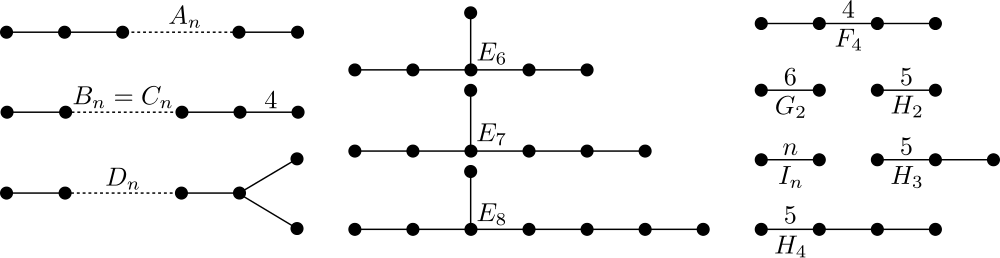
\includegraphics[width=\textwidth]{img/finite-groups.png}
\end{center}

(Image via Wikipedia. We denote $I_2(n)$ instead of $I_n$. Note that $I_2(3)
= A_2$, $I_2(4) = B_2$, $I_2(5) = H_2$, $I_2(6) = G_2$; in particular, we need
not consider $H_2$ or $G_2$ separately. Note that $A_n, B_n, D_n$ each contain
$n$ vertices.)

That is, we will show that any graph not in this list must have one of the
graphs from Lemma \ref{lem15} as a subgraph.
Moreover, we will see that none of the graphs from Lemma \ref{lem15} are
subgraphs of these.

It will remain to show that these
graphs are indeed positive definite.
\\

{\em Proof.}
Make the following observations:

\begin{itemize}
\item
Because $\widetilde{D}_n$ is not an admissible subgraph, we can have at most
one branch point (vertex of degree $>2$).
\item
Because $\widetilde{A}_{n-1}$ is not admissible, we cannot have cycles or
$\infty$ labels.
\end{itemize}

This leaves us with two types of graphs: linear chains, and graphs with
a single branch point.
\\

We continue the proof in the next lecture.


\appendix

\chapter{Version History}
Below we describe briefly the version history of this document, based on
versions which have been published at \url{\thisurl}. Version numbers will
roughly follow the format v0.$n$.$m$, where $n$ indicates the number of
lectures which notes have been written for, and $m$ indicates the number of
minor revisions. Once notes have been taken for all lectures, the version
number will increment to v1.0.

\begin{enumerate}
\item[\bf v0.3.0:] Initial publication with lectures 1 to 3, \S1.1-1.3.
\end{enumerate}


\end{document}
